\documentclass[11pt,a4paper,italian]{article}

\usepackage{graphicx}

\usepackage{titlesec}

\usepackage{tikz, pgfplots}

\pgfplotsset{compat=1.17}

\usepackage[none]{hyphenat}

\usepackage{amssymb}

\usepackage{amsmath}

\numberwithin{equation}{section}

\usepackage{multicol}

\usepackage[margin=1.2in]{geometry}

\usepackage{fancyhdr}

\pagestyle{fancy}

\fancyhead[RO,LE]{\textbf{Introduzione alla fisica dei sistemi complessi}}

\fancyhead[LO,RE]{Luca Morelli}


\titleformat{\section}[display]
{\raggedleft\bfseries\LARGE\narrower\narrower}
{\raggedleft\Huge\normalfont\textbf{{\rlap{ \resizebox{!}{1.2cm}{\thesection} \textcolor{blue}{\rule{17cm}{1.2cm}}} }}}
{0pt}{}

\titleformat{\paragraph}[margin]
{\filleft\bfseries\narrower\narrower}
{\thesection }
{0.5em}{}


\titlespacing{\paragraph}
{7pc}{1.5ex plus .1ex minus .2ex}{1pc}

\renewcommand*\contentsname{Contenuti}
\renewcommand*\refname{Bibliografia}
\renewcommand*\figurename{Figura}

\begin{document}

\begin{titlepage}
	\vspace*{5cm}
	\begin{center}
	\huge \textbf{Differential geometry}
	
	\rule{7cm}{0.4pt} 
	
	\LARGE A brief guide for general relativity
	
	\vspace{40pt}
	
	\LARGE \textbf{Luca Morelli}
	
	\vspace{20pt}
	
	\LARGE March 2024
	
	\end{center}
   
   \vspace{200pt}
   
    \begin{flushright}
    	Citazione a piè pagina
    	
    	perchè comunque fa figo
    	
    	e noi la mettiamo.
    \end{flushright}	
\end{titlepage}

\begin{titlepage}
\begin{center}
	\textbf{Prefazione:}
\end{center}

Questi appunti nascono come una mia personale riformulazione di quelli presi a lezione e quindi soffrono di tutti quei problemi che possono sorgere durante l'operazione di prendere note di quanto viene spiegato. Non sarà quindi raro trovare errori ed imprecisioni dovuti al fatto che prima di poter riportare gli argomenti del corso in questa forma ho dovuto comprenderli io. \\

Inoltre bisogna ricordare che questo è solamente un corso introduttivo atto a presentare un corso di laurea magistrale e che quindi non può avere la pretesa di essere esaustivo e completo. Molti argomenti infatti sono trattati con poco rigore e più con l'intuizione che dovrebbe caratterizzare un fisico nel suo primo approccio ad una materia. Mi sono inoltre permesso di riordinare gli argomenti trattati secondo la loro pertinenza che io ho osservato, per cui non è detto che sia la migliore.\\

In ultima battuta mi scuso per gli errori di forma e di grammatica che potrebbero apparire, dovuti probabilmente ad una mia maggior concentrazione sui temi matematico-fisici trattati a discapito della forma in cui sono riuscito a riportarli. 
\end{titlepage}

\tableofcontents

\section{Introduzione}

Fino ad ora la fisica è riuscita a descrivere moltissimi fenomeni con l'uso di due approcci diametralmente opposti: da un lato riusciamo a descrivere con estrema precisione sistemi estremamente semplici, come avviene in meccanica, dall'altro sistemi molto complessi con un'approccio statistico, come avviene in termodinamica e in meccanica statistica. \\

Siamo infatti in grado di descrivere perfettamente l'orbita della Terra attorno al Sole fin tanto consideriamo un sistema a due corpi ma nel momento in cui aggiungiamo per esempio l'interazione con la Luna incappiamo nel \textbf{problema dei tre corpi} che non è risolvibile analiticamente ma può essere risolto con metodi di calcolo numerico al calcolatore.\\

Proseguendo aumentando il numero di corpi in questione non siamo nemmeno più in grado di sottoporre il problema alla risoluzione del calcolatore, come avviene nel caso delle molecole di un gas. Siamo però capaci di descrivere statisticamente un gas tramite l'analisi \textbf{all'equilibrio} della sua pressione, della sua temperatura e del suo volume. 

Proprio nella zona di grigio tra queste due casistiche entra in gioco la \textbf{fisica dei sistemi complessi}.
\subsection{Cos'è la complessità}

Come già anticipato parliamo di \textbf{complessità} quando vogliamo descrivere la dinamica di un sistema che presenta:

\begin{itemize}
	\item Molti gradi di libertà
	\item Interazione non trascurabile tra le parti
	\item Troppe condizioni iniziali da conoscere 
\end{itemize}

Per far questo costruiamo un modello che deve essere messo alla prova con la realtà sperimentale e che ci consenta di studiarla matematicamente.

Un esempio di questi si sistemi da modellizzare può essere l'evoluzione di una popolazione o di una pandemia.


\section{L'Equazione Logistica}

L'equazione logistica è un modello matematico adatto a descrivere una vasta gamma di fenomeni, inoltre è estremamente semplice per cui risulta molto utile per introdurre varie considerazioni di base che possiamo fare nello studio di un fenomeno.

\subsection{Il modello}

Consideriamo un popolazione di cui vogliamo studiare la dinamica: cerchiamo quindi di modellizzarla molto semplicemente, per farlo possiamo utilizzare un \textbf{automa cellulare}.\\

Per prima cosa possiamo discretizzare lo spazio dove vive la popolazione e il tempo con cui evolve. Per farlo costruiamo una tabella in cui ogni cella può essere occupata da un individuo e la facciamo evolvere applicando delle regole stabilite ogni $\Delta t$.
\begin{center}
	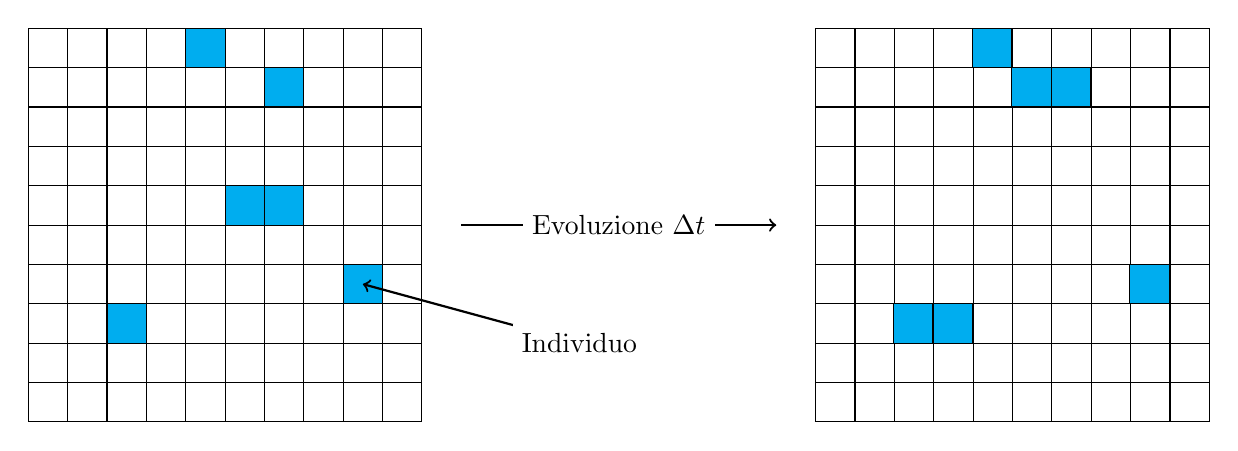
\begin{tikzpicture}
		\draw[step=0.5cm] (0,0) grid (5,5);
		\draw[step=0.5cm] (9.99,0) grid (15,5);
		
		\filldraw[fill=cyan] (1,1) rectangle (1.5,1.5);
		\filldraw[fill=cyan] (3,4) rectangle (3.5,4.5);
		\filldraw[fill=cyan] (4,1.5) rectangle (4.5,2);
		\filldraw[fill=cyan] (2,4.5) rectangle (2.5,5);
		\filldraw[fill=cyan] (2.5,2.5) rectangle (3,3);
		\filldraw[fill=cyan] (3,2.5) rectangle (3.5,3);
		
		\draw[->,thick] (5.5,2.5) -- (9.5,2.5);
		\node[fill=white] at (7.5,2.5) {Evoluzione $\Delta t$};
		
		\filldraw[fill=cyan] (10.99,1) rectangle (11.49,1.5);
		\filldraw[fill=cyan] (12.99,4) rectangle (13.49,4.5);
		\filldraw[fill=cyan] (13.99,1.5) rectangle (14.49,2);
		\filldraw[fill=cyan] (11.99,4.5) rectangle (12.49,5);
		\filldraw[fill=cyan] (12.49,4) rectangle (12.99,4.5);
		\filldraw[fill=cyan] (11.49,1) rectangle (11.99,1.5);
		
		\draw[<-,thick] (4.25,1.75) -- (7,1);
		\node[fill=white] at (7,1) {Individuo};
	\end{tikzpicture}
\end{center}
Le regole che descrivono le dinamiche caratteristiche del sistema sono in questo caso di \textbf{riproduzione-competizione}:

\begin{itemize}
	\item \textbf{Riproduzione}: un individuo si può riprodurre ogni $\Delta t$ se nelle celle adiacenti non ci sono individui con cui competere per il cibo.
	\item \textbf{Competizione}: se un individuo è circondato da troppi contendenti allora muore.
\end{itemize}

Questa tipologia di modello può quindi essere simulata al computer, per poterne facilitare lo studio. Infatti la discretizazione da un lato diminuisce l'aderenza del modello con la realtà ma lo rende più adatto alla simulazione.\\

A questo punto cerchiamo di tradurre il modello in termini matematici. Se chiamiamo $n(t)$ la popolazione al tempo $t$ è immediato dedurre che:

\begin{itemize}
	\item $\Delta n_{Riproduzione} \ \propto \ n(t)$
	\item $\Delta n_{Competizione} \ \propto \ -n^2(t)$
\end{itemize}

Infatti ogni individuo può potenzialmente riprodursi, per cui gli individui nati dopo un $\Delta t$ è maggiore tanto quanto lo sono gli individui totali. Un individuo può invece competere con $n-1$ individui, ossia tutti gli altri, ma poichè gli individui totali sono $n$ allora in totale quelli morti dopo un $\Delta t$ sono proporzionali alle possibili coppie di interazione $n(n-1)\sim n^2$, per cui possiamo scrivere:

\begin{equation}
	n(t+\Delta t)=n(t)+(an(t)-bn^2(t))\Delta t
	\label{logDisc}
\end{equation}

Se consideriamo $\Delta t$ piccolo possiamo passare al continuo ottenendo dalla (\ref{logDisc}) l'\textbf{equazione logistica}:

\begin{equation}
\dot{n}(t)=an(t)(1-\frac{b}{a}n(t)) \label{logequation}
\end{equation}

\subsection{Studio del modello}

Dopo aver ricavato l'equazione che regola il modello possiamo passare ad uno studio matematico procedendo per punti:

\begin{enumerate}
	\item \textbf{In quale spazio mi muovo?} In questo caso $n(t)\in\mathbb{R}^+$
	\item \textbf{Quali sono i punti di equilibrio?} Equilibrio $\Longleftrightarrow$ $\dot{n}(t)=0$ \\ In questo caso abbiamo che $n_{eq}= 0 $ oppure $ n_{eq}= \frac{a}{b}$.
	\item \textbf{Gli equilibri sono stabili o instabili?} \\ Per studiare gli equilibri perturbiamo la soluzione all'equilibrio e studiamo cosa accade alla soluzione:
	\begin{equation}
		\delta n=n(t)-n_{eq} \ \Rightarrow \ \delta \dot{n}=\dot{n}(t)=an(t)(1-\frac{b}{a}n(t))
		\label{logPerturb}
	\end{equation}
     Sostituendo $\delta n$ al posto di $n(t)$ in tutta la (\ref{logPerturb}) troviamo un'equazione differenziale che possiamo linearizzare per studiarla nell'intorno dell'equilibrio.
     \begin{equation}
     	\delta \dot{n}=a(\delta n- n_{eq})-b(\delta n- n_{eq})^2\sim (a-2bn_{eq})\delta n+an_{eq}-bn^2_{eq}
     \end{equation}
 Risulta quindi immediato che se $n_{eq}=0$ allora $\delta n(t)=\delta n_0 e^{at}$, ossia che è un punto di equilibrio instabile, poichè le perturbazioni si allontanano dall'equilibrio. Se $n_{eq}=\frac{a}{b}$ allora la soluzione sarà  $\delta n(t)=\delta n_0 e^{-at}$, per cui la perturbazione tende a convergere sul punto di equilibrio che è quindi stabile.
\end{enumerate}

\subsection{Leggi di scala}

Un'ultima osservazione che possiamo fare sulla (\ref{logequation}) riguarda come riscalano la popolazione e il tempo e come cambia l'equazione. Poniamo quindi il seguente \textbf{riscalamento}:

\begin{equation}
	t\longrightarrow\mu t \qquad n\longrightarrow\lambda n
\end{equation}
applicandolo alla (\ref{logequation}) otteniamo :
\begin{equation}
	\dot{n}(t)=an(t)(1-\frac{b}{a}n(t))\longrightarrow\dot{n}(t)=\mu an(t)-b\mu \lambda n^2(t))
\end{equation}
che osserviamo ridursi ad un'equazione senza parametri se $\mu=a^{-1}$ e $\lambda=\frac{a}{b}$. Questo ci suggerisce che i parametri $a$ e $b$ non sono intrinsecamente importanti per lo studio del modello e che quindi sono solamente le condizioni iniziali a influenzare la soluzione. 
\subsection{La soluzione analitica}
Per terminare ricaviamo la soluzione analitica dell'equazione logistica, per farlo integriamo per parti l'equazione priva di coefficienti, che come abbiamo mostrato con gli opportuni riscalamenti possono essere reintrodotti:
\begin{center}
	
\begin{equation*}
	\begin{gathered}
		\dot{x}=x(1-x)\qquad \Rightarrow \qquad \int_{x_0}^x \frac{ds}{s(1-s)}=\int_0^tdu\\\\
		\int_{x_0}^x \left[ \frac{1-s}{s(1-s)}+\frac{s}{s(1-s)} \right]ds=\int_{x_0}^x \left[ \frac{1}{s}+\frac{1}{(1-s)} \right]ds=t\\\\
		\log\frac{x}{x_0}-\log\frac{1-x}{1-x_0}=\log\frac{x}{1-x} - \log\frac{x_0}{1-x_0}=t\\\\	
		\frac{x}{1-x}=\frac{x_0}{1-x_0}e^t
	\end{gathered}
\end{equation*}

\end{center}\paragraph{Funzione Logistica}
Con un po' di algebra e raccogliendo tutte le costanti in una unica si ottiene la \textbf{funzione logistica}:

\begin{center}
	\begin{equation}
	x(t)=\frac{ce^t}{1+ce^t}
	\label{logfunction}
\end{equation}


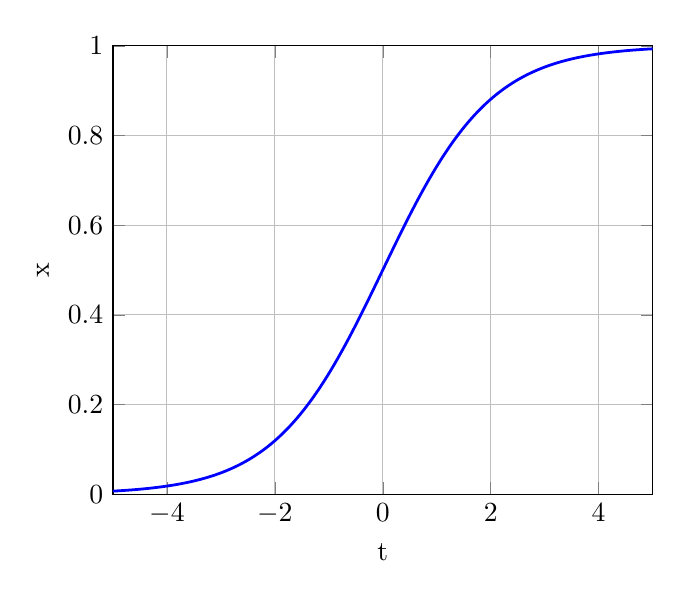
\begin{tikzpicture}
	\begin{axis}[xmin = -5, xmax = 5,
		ymin = 0, ymax = 1,
		grid, xlabel = t, ylabel = x,
		samples=500
		]
		\addplot[% opzioni di disegno
		color=blue, line width=1pt
		] {
			exp(x)/(1+exp(x)) % espressione matematica
		};
	\end{axis}
    \label{graph}
\end{tikzpicture}
\end{center}
Osserviamo che la funzione trovata ha effettivamente il comportamento atteso: cresce esponenzialmente da $x=0$ (eq. instabile) per poi decrescere esponenzialmente verso il valore massimo $x=1$ (eq. stabile). 

\section{Interconnessione di sistemi}

Possiamo modellizzare sistemi complessi costituiti dall'interazione di molti sistemi dinamici, a tale scopo risulta fondamentale comprendere come si struttura la connessione di più sistemi tra di loro.\\

Consideriamo una serie di \textbf{n} sistemi (\textbf{nodi}) che vogliamo collegare con una serie di \textbf{link} di lunghezza \textbf{d}. Se ogni nodo, che potrebbe per esempio essere la cellula di un organismo, ha una dimensione lineare \textbf{l} e il sistema totale, nel nostro esempio l'organismo, ha dimensione lineare \textbf{L} possiamo definire un \textbf{fattore di scala M} che stima quanti nodi sono presenti nel sistema quando il loro numero è nell'ordine della complessità:
\paragraph{Fattore di scala}
\begin{multicols}{2}
	\begin{center}
		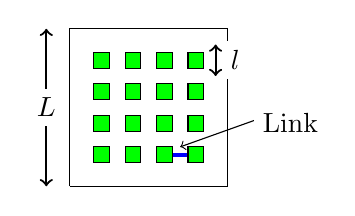
\begin{tikzpicture}
			\draw[step=0.1cm] (0.2,0) -- (0.2,2) -- (2.2,2) -- (2.2,0) -- (0.2,0);
			\draw[thick, <->] (-0.1,0) -- (-0.1,2);
			\node[fill=white] at (-0.1,1) {$L$};
			
			\draw[ultra thick,draw=blue] (1.4,0.4) -- (1.8,0.4);
			
			\filldraw[fill=green, draw=black] (0.5,0.3) rectangle (0.7,0.5);
			\filldraw[fill=green, draw=black] (0.9,0.3) rectangle (1.1,0.5);
			\filldraw[fill=green, draw=black] (1.3,0.3) rectangle (1.5,0.5);
			\filldraw[fill=green, draw=black] (1.7,0.3) rectangle (1.9,0.5);
			
			\filldraw[fill=green, draw=black] (0.5,0.7) rectangle (0.7,0.9);
			\filldraw[fill=green, draw=black] (0.9,0.7) rectangle (1.1,0.9);
			\filldraw[fill=green, draw=black] (1.3,0.7) rectangle (1.5,0.9);
			\filldraw[fill=green, draw=black] (1.7,0.7) rectangle (1.9,0.9);
			
			\filldraw[fill=green, draw=black] (0.5,1.1) rectangle (0.7,1.3);
			\filldraw[fill=green, draw=black] (0.9,1.1) rectangle (1.1,1.3);
			\filldraw[fill=green, draw=black] (1.3,1.1) rectangle (1.5,1.3);
			\filldraw[fill=green, draw=black] (1.7,1.1) rectangle (1.9,1.3);
			
			\filldraw[fill=green, draw=black] (0.5,1.5) rectangle (0.7,1.7);
			\filldraw[fill=green, draw=black] (0.9,1.5) rectangle (1.1,1.7);
			\filldraw[fill=green, draw=black] (1.3,1.5) rectangle (1.5,1.7);
			\filldraw[fill=green, draw=black] (1.7,1.5) rectangle (1.9,1.7);
			
			\draw[thick, <->] (2.05,1.4) -- (2.05,1.8);
			\node[fill=white] at (2.3,1.6) {$l$};
			
			\draw[ <-] (1.6,0.5) -- (3,1);
			\node[fill=white] at (3,0.81) {Link};
			
			
			
		\end{tikzpicture}
	
	\begin{equation}
		M=\left(\frac{L}{l}\right)^D \label{fattoreDiScalaInterconnessioni}
	\end{equation}
\end{center}
\end{multicols}
\vspace{20pt}
dove D è la dimensione del sistema (1D, 2D, 3D).\\

A questo punto possiamo iniziare a stimare il \textbf{costo} di una certa configurazione di link, ossia, se immaginiamo di trasportare un flusso $\Phi$, per esempio di energia o di corrente o di acqua, con il nostro sistema di link, quanto flusso è necessario perchè ogni nodo sia rifornito. \\
Supponiamo quindi che ad ogni nodo si impieghi una quantità $\phi$ di flusso e definiamo il costo del link i-esimo $d\cdot \phi$. Siamo a questo punto costretti ad analizzare l'esempio più semplice di rete per poter comprendere come avviene la sua analisi.

\subsection{Modello lineare}
\begin{center}
	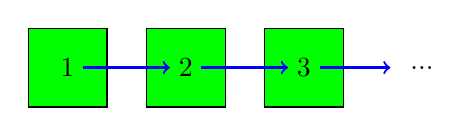
\begin{tikzpicture}
		\filldraw[fill=green,draw=black] (0,0) rectangle (1,1);
		\node[fill=green] at (0.5,0.5) {1};
		\filldraw[fill=green,draw=black] (1.5,0) rectangle (2.5,1);
		\node[fill=green] at (2,0.5) {2};
		\filldraw[fill=green,draw=black] (3,0) rectangle (4,1);
		\node[fill=green] at (3.5,0.5) {3};
		\draw[->,thick, draw=blue] (0.7,0.5) -- (1.8,0.5);
		\draw[->,thick, draw=blue] (2.2,0.5) -- (3.3,0.5);
		\draw[->,thick, draw=blue] (3.7,0.5) -- (4.6,0.5);
		\node[fill=white] at (5,0.5){...};
	\end{tikzpicture}\\
\end{center}



Immaginiamo di collegare ogni nodo uno dopo l'altro a catena, per quanto abbiamo detto il flusso all'i-esimo nodo sarà $\Phi_i=\Phi_{i-1}-d\cdot \phi$. Per cui se il numero di nodi è stimabile con M il costo totale sarà:
\begin{align*}
	\sum^M_{k=1} d\cdot \phi\cdot k = d\cdot \phi\cdot \sum^M_{k=1} k=\frac{M(M-1)}{2}d\cdot \phi\backsimeq\frac{d\cdot\phi}{2}M^2
\end{align*} 
che utilizzando la (\ref{fattoreDiScalaInterconnessioni}) e ricorando che $L^3$ è circa il volume del sistema, il nostro modello prevede che, nel caso in cui le dimensioni dei nodi e dei link non varino ma aumentino solamente il loro numero, il costo del sistema di interconnessione aumenta con il quadrato del volume del corpo.
\begin{equation}
	Costo=\frac{d\cdot\phi}{2\cdot l^6}V^2
\end{equation}

\subsection{Modello ad albero}
\begin{center}
	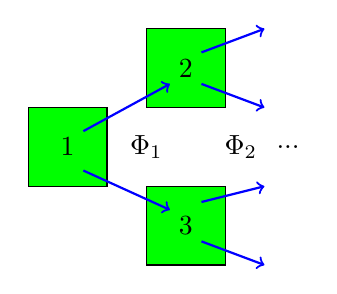
\begin{tikzpicture}
		\filldraw[fill=green,draw=black] (0,0) rectangle (1,1);
		\node[fill=green] at (0.5,0.5) {1};
		\filldraw[fill=green,draw=black] (1.5,1) rectangle (2.5,2);
		\node[fill=green] at (2,1.5) {2};
		\filldraw[fill=green,draw=black] (1.5,0) rectangle (2.5,-1);
		\node[fill=green] at (2,-0.5) {3};
		\draw[->,thick, draw=blue] (0.7,0.7) -- (1.8,1.3);
		\draw[->,thick, draw=blue] (0.7,0.2) -- (1.8,-0.3);
		\draw[->,thick, draw=blue] (2.2,1.7) -- (3,2);
		\draw[->,thick, draw=blue] (2.2,1.3) -- (3,1);
		\draw[->,thick, draw=blue] (2.2,-0.2) -- (3,0);
		\draw[->,thick, draw=blue] (2.2,-0.7) -- (3,-1);
		\node[fill=white] at (2.7,0.5) {$\Phi_2$};
		\node[fill=white] at (1.5,0.5) {$\Phi_1$};
		\node[fill=white] at (3.3,0.5){...};
	\end{tikzpicture}\\
\end{center}

In questo caso colleghiamo i nodi biforcando le connessioni ad ogni nodo in maniera tale che il flusso i-esimo risulti $\Phi_i=\frac{\Phi_{i-1}-\phi\cdot d}{2}$.

Questo sarebbe il comportamento ideale e più efficiente ma è possibile dimostrare che non è realizzabile.

\subsection{Modello a raggiera}
\begin{center}
	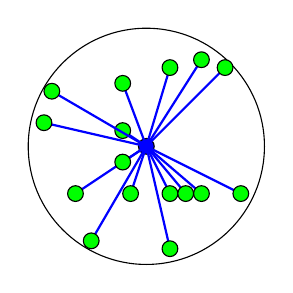
\begin{tikzpicture}
		\draw (0,0) circle (1.5cm);
		\filldraw[fill=blue] (0,0) circle (0.1cm);
		\draw[draw=blue, thick] (0,0) -- (1,1);
		\filldraw[fill=green] (1,1) circle (0.1cm);
		\draw[draw=blue, thick] (0,0) -- (0.3,-0.6);
		\filldraw[fill=green] (0.3,-0.6) circle (0.1cm);
		\draw[draw=blue, thick] (0,0) -- (-0.3,0.2);
		\filldraw[fill=green] (-0.3,0.2) circle (0.1cm);
		\draw[draw=blue, thick] (0,0) -- (-0.9,-0.6);
		\filldraw[fill=green] (-0.9,-0.6) circle (0.1cm);
		\draw[draw=blue, thick] (0,0) -- (0.3,1);
		\filldraw[fill=green] (0.3,1) circle (0.1cm);
		\draw[draw=blue, thick] (0,0) -- (0.7,-0.6);
		\filldraw[fill=green] (0.7,-0.6) circle (0.1cm);
		\draw[draw=blue, thick] (0,0) -- (-0.3,0.8);
		\filldraw[fill=green] (-0.3,0.8) circle (0.1cm);
		\draw[draw=blue, thick] (0,0) -- (-0.3,-0.2);
		\filldraw[fill=green] (-0.3,-0.2) circle (0.1cm);
		
		\draw[draw=blue, thick] (0,0) -- (-1.2,0.7);
		\filldraw[fill=green] (-1.2,0.7) circle (0.1cm);
		\draw[draw=blue, thick] (0,0) -- (1.2,-0.6);
		\filldraw[fill=green] (1.2,-0.6) circle (0.1cm);
		\draw[draw=blue, thick] (0,0) -- (0.7,1.1);
		\filldraw[fill=green] (0.7,1.1) circle (0.1cm);
		\draw[draw=blue, thick] (0,0) -- (-0.2,-0.6);
		\filldraw[fill=green] (-0.2,-0.6) circle (0.1cm);
		\draw[draw=blue, thick] (0,0) -- (0.3,-1.3);
		\filldraw[fill=green] (0.3,-1.3) circle (0.1cm);
		\draw[draw=blue, thick] (0,0) -- (0.5,-0.6);
		\filldraw[fill=green] (0.5,-0.6) circle (0.1cm);
		\draw[draw=blue, thick] (0,0) -- (-1.3,0.3);
		\filldraw[fill=green] (-1.3,0.3) circle (0.1cm);
		\draw[draw=blue, thick] (0,0) -- (-0.7,-1.2);
		\filldraw[fill=green] (-0.7,-1.2) circle (0.1cm);
		
	\end{tikzpicture}
\end{center}

Colleghiamo in questo caso ogni nodo con un singolo link, allora la lunghezza media dei link è confrontabile con la dimensione lineare del sistema per cui il costo è facilmente stimato come:
\begin{equation}
	Costo\ \sim M \phi L \sim \phi M^{\frac{D+1}{D}} 
\end{equation}
ricordando che $L^D\sim M$.\\

Osserviamo subito che in questo caso se il sistema si distribuisce linearmente o su una superficie, come una città, o nello spazio, come il corpo umano, questo modifica sensibilmente la forma analitica del costo. Infatti se $D=1$ otteniamo un dipendenza quadratica da $L$, mentre su una superficie abbiamo una dipendenza come $x^{\frac{3}{2}}$ dall'area occupata e per $D=3$ abbiamo:
\begin{equation}
	Costo\ \sim \phi V^{\frac{4}{3}} \label{modelloRaggieraTeorico}
\end{equation}

Questo modello si rivela essere il migliore sistema logistico realizzabile da un punto di vista teorico. In realtà però si scopre che non è il modello che la natura ha scelto per gli organismi viventi per esempio. 
\paragraph{Legge di Kleiber}
Si scopre infatti che la massa corporea, quindi il volume, di un organismo è legato alla potenza dissipata dal metabolismo basale da una legge a potenza nella forma:
\begin{equation}
	P\sim V^{\frac{3}{4}}
\end{equation}
che è molto differente dalla legge che abbiamo ricavato, il che ci suggerisce che la natura tiene conto anche di altri fattori per lo sviluppo delle reti logistiche negli organismi.

\section{Il neurone: un sistema del second'ordine}

In questo capitolo studieremo un modello descritto da un'\textbf{equazione differenziale del secondo ordine}, che può essere utilizzato per descrivere vari sistemi che reagiscono a stimoli oltre una certa soglia, ma che può rivelarsi estremamente utile per acquisire nuovi strumenti per l'analisi delle equazioni differenziali più complesse.

\subsection{Comportamenti con soglia} 

Consideriamo un oscillatore armonico sottoposto a smorzamento:
\begin{equation}
	\ddot{x}=-x-\gamma\dot{x} \label{oscillatoreSmorzato}
\end{equation}
vogliamo modificare questa equazione affinchè il comportamento del sistema dipenda fortemente da $x$, nella fattispecie vogliamo modulare lo smorzamento. 

Osserviamo che possiamo modificare il segno del termine di smorzamento per annullarne gli effetti sul sistema. Modifichiamo quindi la (\ref{oscillatoreSmorzato}) con un termine aggiuntivo $1-x^2$ che per $x$ piccolo è positivo ma cambia di segno per $x>1$. Otteniamo quindi: 
\begin{equation}
	\ddot{x}=-x-\gamma(1-x^2)\dot{x} \label{pendoloSoglia}
\end{equation}
questo tipo di sistema è caratterizzato da un comportamento di smorzamento dipendente dalla posizione, per cui oltre un valore soglia, quando $x>1$ il termine di smorzamento cambia segno e il sistema dissipa energia (meccanicamente parlando) e inizia a tendere a $x=0$.

Osserviamo che per $\gamma<0$ si manifesta il comportamento opposto, ossia che oltre un valore soglia il sistema inizia ad assorbire energia e la sua soluzione diverge dalle condizioni iniziali verso infinito.\\

In ogni caso il termine aggiuntivo è in grado, variando il segno di una parte dell'equazione, di introdurre una soglia oltre la quale il comportamento del sistema muta. 

\subsection{Riduzione al prim'ordine}

Il termine moltiplicativo che abbiamo aggiunto ha però lo svantaggio di rendere più complessa la risoluzione dell'equazione differenziale (\ref{pendoloSoglia}).\\

Introduciamo una nuova variabile per poter ridurre l'ordine dell'equazione differenziale aumentandone la dimensione:
\begin{equation*}
	\dot{y}=-\frac{x}{\gamma} \Rightarrow  \ddot{x}=\gamma \dot{y}-\gamma(1-x^2)\dot{x} 
\end{equation*}

Integrando otteniamo il sistema:
\begin{equation}
	\begin{cases}
		\dot{x}=\gamma y+\gamma(x-\frac{x^3}{3})\\
		\dot{y}=-\frac{x}{\gamma}
		\label{sistema}
	\end{cases}
\end{equation}

Dobbiamo quindi studiare il sistema (\ref{sistema}) per poter comprendere meglio le proprietà del modello. Come già fatto per l'equazione logistica iniziamo studiando i punti di equilibrio, ossia quando $\dot{x}=0$ e $\dot{y}=0$; ogni singola condizione definisce in una sorta di spazio delle fasi $(x,y)$ i luoghi dei punti in cui il sistema è in equilibrio rispetto ad $x$ o $y$, queste curve sono dette \textbf{nullcline}, dall'inglese \emph{nullclines}, e risulteranno fondamentali per comprendere qualitativamente l'evoluzione del sistema.
\begin{multicols}{2}
	\begin{center}
	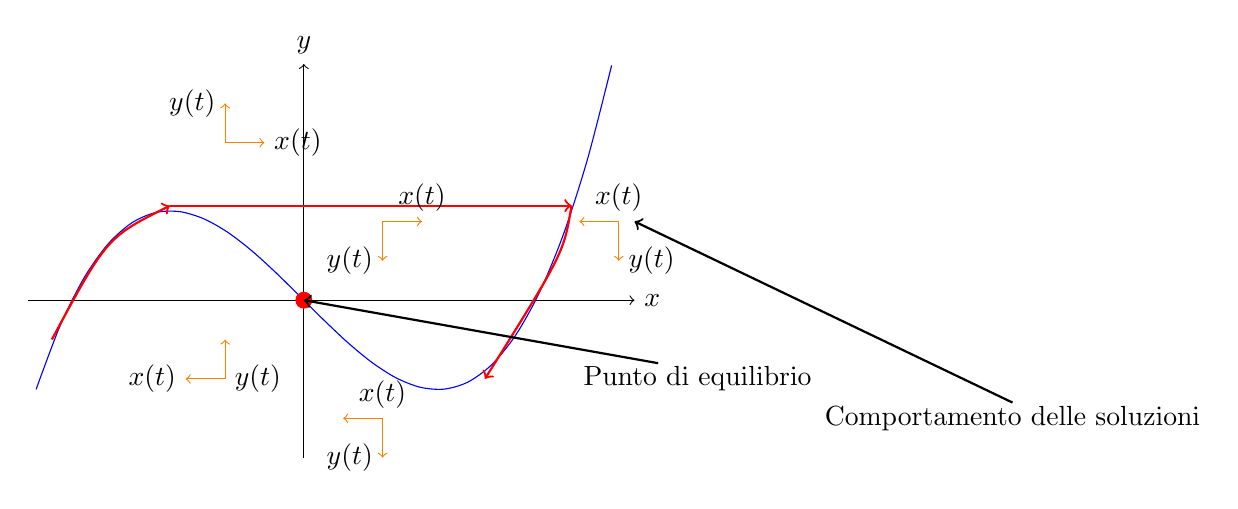
\begin{tikzpicture}
			\draw[->] (-3.5, 0) -- (4.2, 0) node[right] {$x$};
			\draw[->] (0, -2) -- (0, 3) node[above] {$y$};
			\draw[scale=1.7, domain=-2:2.3, smooth, variable=\x, blue] plot ({\x}, {-\x+\x*\x*\x/3});
			
			\draw[draw=red, thick, ->] (-3.2,-0.5) .. controls (-2.5,0.8) .. (-1.7,1.2);
			\draw[draw=red, thick, ->] (-1.7,1.2) -- (3.4,1.2);
			\draw[draw=red, thick, ->] (3.4,1.2) .. controls (3.3,0.6) .. (2.3,-1);
			
			\draw[draw=orange,->] (1,1) -- (1.5,1) node[above] {$x(t)$};
			\draw[draw=orange,->] (1,1) -- (1,0.5) node[left] {$y(t)$};
			\draw[draw=orange,<-] (3.5,1) -- (4,1) node[above] {$x(t)$};
			\draw[draw=orange,->] (4,1) -- (4,0.5) node[right] {$y(t)$};
			\draw[draw=orange,<-] (0.5,-1.5) -- (1,-1.5) node[above] {$x(t)$};
			\draw[draw=orange,->] (1,-1.5) -- (1,-2) node[left] {$y(t)$};
			\draw[draw=orange,->] (-1,-1) -- (-1.5,-1) node[left] {$x(t)$};
			\draw[draw=orange,<-] (-1,-0.5) -- (-1,-1) node[right] {$y(t)$};
			\draw[draw=orange,->] (-1,2) -- (-0.5,2) node[right] {$x(t)$};
			\draw[draw=orange,->] (-1,2) -- (-1,2.5) node[left] {$y(t)$};
			
			\filldraw[draw=red,fill=red] (0,0) circle (0.1cm);
			\draw[thick, <-] (0,0) -- (4.5,-0.8);
			\node[] at (5,-1) {Punto di equilibrio};
			\draw[thick, <-] (4.2,1) -- (9,-1.3);
			\node[] at (9,-1.5) {Comportamento delle soluzioni};
			
	\end{tikzpicture}
\end{center}
\begin{align*}
	Nullcline\quad\Rightarrow\quad
	\begin{cases}
			x=0\\
		y=\frac{x^3}{3}-x
	\end{cases}\\
	\begin{cases}
		x>0\quad \Rightarrow \quad \dot{y}<0\\
		y>\frac{x^3}{3}-x \quad \Rightarrow \quad \dot{x}>0
	\end{cases}
\end{align*}

\end{multicols}	

Osserviamo subito che il punto di equilibrio complessivo del sistema è dato dall'intersezione delle nullcline, poiché in questi punti sia $\dot{x}$ e $\dot{y}$ si annullano: nel nostro caso questo avviene nell'origine.\\

In secondo luogo osserviamo che le nullcline separano il piano in due regioni ciascuna, ognuna dove la variabile della nullclina cresce o decresce, infatti annullandosi $\dot{x}$ e $\dot{y}$ sulle curve abbiamo che queste delimitano le regioni dove $\dot{x}$ e $\dot{y}$ hanno segni diversi e quindi dove varia la monotonia della soluzione.\\

Definiamo ora \textbf{variabile veloce} la variabile che cresce più rapidamente nella dinamica del sistema e conseguentemente definiamo la \textbf{variabile lenta}.\\ In questo caso è semplice distinguerle infatti sappiamo che $\dot{y}=-\frac{x}{\gamma}$, il che per $\gamma$ grandi rende molto più lenta la crescita di $y$ rispetto a quella di $x$, che infatti è la variabile veloce. Per lo studio del sistema riconoscere queste differenze è fondamentale infatti il sistema cercherà di evolvere seguendo la dinamica della variabile veloce e, ove è possibile, la sua nullclina. \\

Infine osserviamo che il moto sulla nullclina veloce non sempre è compatibile con la dinamica locale del sistema: immaginiamo di portare il sistema a $x$ e $y$ negativi sulla nullclina di $\dot{x}$, in questo caso $\dot{x}=0$, per cui verrà seguita la dinamica di $y$ sulla nullcina stessa, infatti abbiamo già detto che per $x<0$ si ha che $\dot{y}>0$ per cui il sistema tenderà a risalire verso l'origine del piano. \\
Giunto al primo massimo locale il sistema, per seguire la nullclina, dovrebbe far decrescere $y$, cosa non concessa dalla condizione $\dot{y}>0$. In questo caso è la dinamica veloce di $x$ a spostare il sistema dal punto di massimo alla regione con $x>0$ mantenendo $y$ circa costante, in tempi molto brevi, fino ad incontrare nuovamente la nullclina in un punto dove il moto sulla curva sarà di nuovo concorde con le condizioni locali sulle derivate prime.\\

Questo tipo di comportamento genera un'orbita stabile attorno all'origine che però è un punto di equilibrio instabile poichè è situato in una zona \textbf{proibita} delle nullcline.\\ Se però $\gamma$ fosse stato negativo l'origine sarebbe chiaramente stata un punto stabile, come già osservato all'inizio. Questo tipo di fenomeno attorno ai punti di equilibrio prende il nome di \textbf{Biforcazione di Hopf}. 

\subsection{Il modello del neurone}

Quanto abbiamo appena compreso si rivela utile per la comprensione del modello matematico utilizzato per descrivere la risposta ad impulsi elettrici dei neuroni. Chiamiamo $x$ la tensione nel neurone, $w$ la corrente che vi scorre all'interno e $I$ un ipotetico stimolo esterno che il neurone può ricevere, allora:
\begin{equation}
		\dot{x}=x-\frac{x^3}{3}-w+I \qquad
		\dot{w}=\frac{x+a-bw}{\gamma}
\end{equation} 
Come già abbiamo fatto procediamo a studiare le nullcline, i punti di equilibrio e le variabili del sistema. Chiaramente è $x$ la variabile veloce.
\begin{multicols}{2}
	\begin{center}
		\begin{tikzpicture}
			\draw[->] (-3.5, 0) -- (2.7, 0) node[right] {$x$};
			\draw[->] (0, -2) -- (0, 2) node[above] {$w$};
			\draw[scale=1.7, domain=-2:1.5, smooth, variable=\x, blue] plot ({\x}, {+\x-\x*\x*\x/3-0.5});
			\draw[scale=1.7, domain=-2:1.3, smooth, variable=\x, blue] plot ({\x}, {\x+0.5});
			
			
		\end{tikzpicture}
	\end{center}

    Lo studio delle nullcline evidenzia che esiste un punto di equilibrio, infatti non è possibile costruire le due curve senza che si intersechino, non sappiamo però nulla sulla sua stabilità. \\
    
    Procediamo quindi a studiare le perturbazioni vicino all'equilibrio linearizzando il sistema di equazioni differenziali.
\end{multicols}
\begin{multicols}{2}
\begin{align*}
	\delta x=x-x_{eq} \qquad \qquad \quad \delta w=w-w_{eq}\\
	\delta \dot{x}=(1-x^2_{eq})\delta x-\delta w \qquad \delta \dot{w}=\frac{\delta x -b\ \delta w}{\gamma}
\end{align*}
\begin{align*}
	\\\\
	\begin{pmatrix}
		\dot{x} \\
		\dot{w}
	\end{pmatrix}
	=
	\begin{pmatrix}
		1-x_{eq}^2 & -1 \\
		\frac{1}{\gamma} & -\frac{b}{\gamma}
	\end{pmatrix}
	\begin{pmatrix}
		x \\
		w
	\end{pmatrix}
=
M\begin{pmatrix}
	x \\
	w
\end{pmatrix}
\end{align*}
\end{multicols}
Ora possiamo studiare la traccia e il determinante della matrice che caratterizza il sistema linearizzato per capire quali condizioni rendono entrambi gli autovalori negativi così che le perturbazioni convergano verso il punto di equilibrio.

\begin{align}
\det(M)= -\frac{b}{\gamma}(1-x^2_{eq})+\frac{1}{\gamma}\propto\lambda_1\ \lambda_2\\
Tr (M)=(1-x^2_{eq})-\frac{b}{\gamma}\propto\lambda_1+\lambda_2
\end{align}

Risulta chiaro che per $x_{eq}^2>>0$ gli autovalori sono negativi per cui l'equilibrio è stabile e viceversa per $x_{eq}^2$ che tende a zero.\\

Infine osserviamo che il termine $I$ costituisce un paramento di traslazione verticale per la nullclina di $\dot{x}$, questo quindi regola a che distanza dell'origine è collocato il punto di equilibrio e quindi la sua stabilità. Possiamo però anche vedere questo termine come dipendente dal tempo e nella fattispecie nella forma $\Delta I\ \delta(t)$, ossia del prodotto tra un termine costante e una Delta di Dirac. Così facendo l'integrazione di questo termine ha l'effetto di cambiare le condizioni iniziali del sistema che si troverà lontano dal punto di equilibrio.

A questo punto se $\Delta I$ è grande a sufficienza e il punto di equilibrio è stabile  il sistema inizierà ad orbitare attorno al punto di equilibrio come avviene per il biforcamento di Hopf, ossia separandosi dalla nullclina, in maniera tale da generare una crescita rapida che va poi a decadere nel tempo come risposta allo stimolo esterno. Se $\Delta I$ invece non è sufficientemente grande il sistema oscillerà attorno all'equilibrio senza generare un risposta.
\begin{center}
	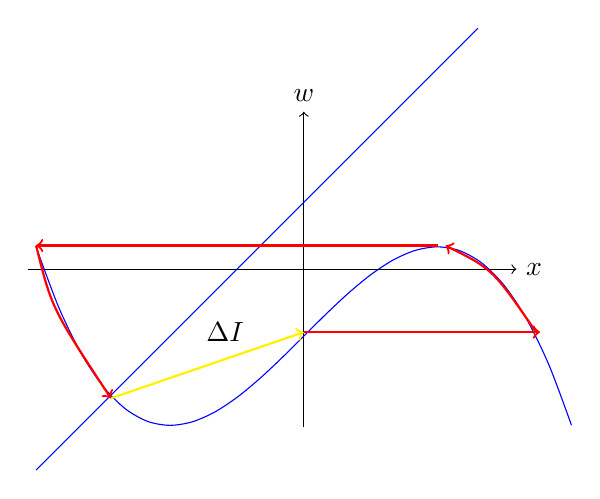
\begin{tikzpicture}
		\draw[->] (-3.5, 0) -- (2.7, 0) node[right] {$x$};
		\draw[->] (0, -2) -- (0, 2) node[above] {$w$};
		\draw[scale=1.7, domain=-2:2, smooth, variable=\x, blue] plot ({\x}, {+\x-\x*\x*\x/3-0.5});
		\draw[scale=1.7, domain=-2:1.3, smooth, variable=\x, blue] plot ({\x}, {\x+0.5});
		
		\draw[thick ,draw=yellow, ->] (-2.45,-1.64) -- (0,-0.8);
		\draw[thick, draw=red, ->] (0,-0.8) -- (3,-0.8) ;
		\draw[thick, draw=red, ->] (2.95,-0.8) .. controls (2.4,0) ..(1.8,0.3);
		\draw[thick, draw=red, ->] (1.7,0.3) -- (-3.4,0.3) ;
		\draw[thick, draw=red, ->] (-3.4,0.3) .. controls (-3.2,-0.5) ..(-2.45,-1.64);
		\node at (-1,-0.8) {$\Delta I$};
		
	\end{tikzpicture}
\end{center}

Abbiamo quindi ottenuto un sistema in grado di rispondere a stimoli esterni con un meccanismo di soglia che nei neuroni è utilizzato per evitare scariche anomale nel sistema nervoso, cosa che per esempio non viene evitata durante un attacco epilettico.



\section{Il modello epidemiologico SIR}

Vogliamo studiare ora la diffusione di una pandemia, per farlo analizzeremo il modello più semplice possibile ossia il modello \textbf{SIR}. Consideriamo una popolazione di \textbf{N} individui fissi, assunzione che possiamo fare se pensiamo di studiare la popolazione per un tempo sufficientemente corto per cui le persone decedute sono approssimativamente compensate da quelle nate. \\
La popolazione è quindi suddivisa in tre sottosistemi \textbf{S}, i suscettibili, \textbf{I}, gli infetti, e \textbf{R}, i recovered ossia i guariti. In questo caso l'assunzione che N sia costante ci consente di introdurre un sorta di \textbf{legge di conservazione}:
\begin{equation}
	S+I+R=N
	\label{continuità}
\end{equation} 
Inoltre dobbiamo definire delle leggi che consentano modellizzare i link tra i tre sottosistemi, queste ovviamente devono rispettare la (\ref{continuità}) e quindi nella loro forma più semplice appaiono come:
\begin{equation}
	\begin{cases}
		\dot{S}=-\Phi_{S\rightarrow I}(t)\\
		\dot{I}=\Phi_{S\rightarrow I}(t)-\Phi_{I\rightarrow R}(t)\\
		\dot{R}=\Phi_{I\rightarrow R}(t)\\
	\end{cases}
\label{flussi}
\end{equation}
Così facendo il problema si sposta sulla necessità di trovare le 3 funzioni dei flussi tra i sottosistemi:
\begin{itemize}
	\item $\Phi_{S\rightarrow I}(t)$ è facilmente definito infatti è chiaro che se ogni individuo può infettarsi allora il flusso sarà dato dal numero di suscettibili per la probabilità che incontrino un infetto, stimata con $\frac{I}{N}$, e per un fattore $m(t)$ che misura la socialità, per cui abbiamo :
	\begin{equation}
		\Phi_{S\rightarrow I}(t)=\beta S\frac{I}{N}m(t)
	\end{equation}
    \item $\Phi_{I\rightarrow R}(t)$ è più complesso da ricavare, infatti deve tenere conto del ritardo dovuto al tempo di guarigione, per farlo consideriamo la seguente espressione:
    \begin{equation}
    	\Phi_{I\rightarrow R}(t)=\int_{0}^{\infty}\Gamma_I(s) \Phi_{S\rightarrow I}(t-s)ds
    \end{equation}
     Questa ci consente di stimare quante persone che si sono infettate al tempo $t-s< t$ guariscono al tempo $t$, moltiplicandole per la probabilità $\Gamma_I(s)$ di guarire dopo un tempo $s$ che sono infette. 
\end{itemize}
\vspace{5pt}

Solitamente la probabilità di guarire è data da una particolare funzione $\Gamma_I(s)=cs^ae^{-bt}$, che chiaramente tende a zero sia per $s$ piccolo che grande, fornendo quindi un punto in qui la probabilità di guarire è massima.\\ Risulta però molto complicato utilizzare questo integrale come definizione del flusso per cui introdurremo una serie di approssimazioni e semplificazioni: in primo luogo considereremo un valore medio della probabilità ($\gamma$) e lo assumeremo costante durante l'integrazione, in secondo luogo supponiamo che $\Phi_{S\rightarrow I}(t)>>\Phi_{I\rightarrow R}(t)$, cosa effettivamente vera durante le prime fasi dell'epidemia, in questo modo possiamo approssimare $\Phi_{S\rightarrow I}(t)\backsimeq\dot{I}$ che se integrato restituisce $I(t)$, poichè per tempi molto precedenti la pandemia non è ancora incominciata e quindi risulta nullo il numero di infetti. Otteniamo quindi dalla (\ref{flussi}) un modello più semplice ma ancora utile:
\begin{equation}
	\begin{cases}
		\dot{S}=-m(t)\beta S\frac{I}{N}\\
		\dot{I}=m(t)\beta S\frac{I}{N}-\gamma I\\
		\dot{R}=\gamma I\\
	\end{cases}
	\label{SIR}
\end{equation}

Prima di iniziare a studiare il modello procediamo a riscalare le variabili in maniera tale da normalizzare la popolazione, imponiamo infatti che $N=1$ e studieremo le variazioni percentuali da qui in poi.
\subsection{Studio del modello}

Per prima cosa osserviamo che se $I=0$ chiaramente il sistema è in equilibrio, per cui studieremo quali condizioni consentono ad una epidemia di svilupparsi e come questo sviluppo avviene.\\

Perchè l'epidemia si diffonda dobbiamo introdurre almeno un infetto, in questo caso però piccole perturbazioni di $I$ lasciano pressochè invariato $S=1$, per cui abbiamo come condizione per lo svilupparsi dell'epidemia:
\begin{equation}
	\dot{I}=(-m_0\beta-\gamma )I \Rightarrow m_0\beta>\gamma
\end{equation} 
ossia che i parametri che influenzano la diffusione devono "\textit{surclassare}" quelli relativi alla guarigione.\\

Posso a questo punto proseguire nello studio osservando che con una semplice sostituzione di variabili è possibile ridurre il modello ad un sistema \textbf{Hamiltoniano} di cui ben conosciamo le caratteristiche:
\begin{equation*}
	\begin{gathered}
		\frac{\dot{S}}{S}=\frac{d}{dt} \log S =-m(t)\beta I\qquad\log S=u\qquad \dot{u}=-m(t)\beta e^{v}=-\frac{\partial\mathcal{H}}{\partial v}\\
			\qquad\qquad\Rightarrow\qquad\\
			\frac{\dot{I}}{I}=\frac{d}{dt}  \log S =m(t)\beta S-\gamma\qquad\log =v\qquad\dot{v}=m(t)\beta e^{u}-\gamma=\frac{\partial\mathcal{H}}{\partial u}\\
	\end{gathered}
\end{equation*}
Così facendo troviamo un integrale primo del moto che ci consentirà di fare alcune osservazioni utili, da qui in poi però dobbiamo assumere che $m(t)$ sia costante:
\begin{equation}
	\mathcal{H}(I,S)=m\beta(I+S)-\gamma\log S=m\beta \label{hamilton}
\end{equation}
Così facendo, conoscendo le condizioni iniziali del sistema e quindi il valore dell'integrale primo, possiamo determinare in quanti punti vale $I=0$ : infatti un primo punto che non ha infetti è il punto iniziale e se vi fosse un secondo punto in tal caso avremo la fine della pandemia. Studiando la  (\ref{hamilton}) si scopre facilmente che la condizione perchè l'epidemia possa avere luogo sono anche sufficienti per la sua fine; in questo caso bisogna risolvere un'equazione non algebrica per cui è necessario uno studio di funzione molto banale che però omettiamo (perchè non ho voglia ed è una cazzata).\\

Vogliamo a questo punto prevedere quando si manifesterà il picco di infetti e comprenderne l'entità. Ricordando, dal cambio variabili di prima, che $\frac{\dot{S}}{S}=\frac{d}{dt} \log S =-m\beta I$, possiamo ridurre la (\ref{hamilton}) alla seguente forma:
\begin{equation*}
	-\frac{\dot{S}}{S} + m\beta S-\gamma\log S=m\beta
\end{equation*}
a questo punto approssimiamo in serie di Taylor $\log S\simeq1-S$ ottenendo così un'equazione differenziale che abbiamo già incontrato, ossia l'equazione logistica, che però è valida solo per $S\sim 1$, ovvero solo se l'epidemia è agli inizi o ad essere infetti non è una percentuale troppo grossa della popolazione (se $S=0,6$ l'errore $\simeq 15\%$).
\begin{equation}
	\dot{S}=(\beta m-\gamma)(1-S)S
\end{equation} 

Infine osserviamo che se $\frac{\dot{S}}{S}=-m\beta I$ e $S\simeq 1$ allora possiamo stimare a grandi linee il punto di massimo di $I$ come il punto di flesso di $S$, infatti:
\begin{equation}
	\dot{I}=\frac{\ddot{S}S-\dot{S}^2}{S^2}=\frac{\ddot{S}}{S}-I^2
\end{equation}
e questa espressione tende a $0$ se $I<<S$ e $\ddot{S}=0$. Questa stima in realtà è del tutto generale e infatti $\frac{\dot{S}}{S}=-m\beta I$ è immediatamente ricavabile dalla (\ref{SIR}).

\section{Sistemi lineari ed interazioni tra sistemi}

I sistemi di equazioni differenziali più semplici che possiamo considerare sono i \textbf{sistemi lineari} e dall'analisi matematica sappiamo che possiamo sempre trovare una soluzione, unica, per questo tipo di equazioni, una volta stabilite le condizioni iniziali.
\begin{equation}
	x\in\mathbb{R}^n \qquad \dot{x}=Ax \qquad \Rightarrow \qquad x(t)=\sum_\lambda v_\lambda \ e^{\lambda t}
\end{equation}
Dove $A$ è una matrice quadrata $n\times n$ e $v_\lambda$ è un suo auto vettore di autovalore $\lambda$.\\

La semplicità di queste soluzioni consentono di stimare l'evoluzione di una perturbazione delle condizioni iniziali $\delta x_0$ ad un tempo $t$:
\begin{equation}
	\|\delta x(t)\| \backsimeq |e^{\lambda t}|\ \|\delta x_0\|
\end{equation}
\paragraph{Esponente di Lyapunov}
dove $\lambda$ è detto \textbf{esponente di Lyapunov} e chiaramente se ha parte reale positiva implica che la perturbazione porterà la soluzione a divergere da quella iniziale.

Possiamo inoltre stimare il \textbf{tempo di predicibilità} del modello come il tempo $t^*$ per cui errori piccoli sulle condizioni iniziali non sono più trascurabili:
\begin{equation}
	\|\delta x_0\| \ |e^{\lambda t^*}|\sim1\qquad\Rightarrow\qquad t^*=-\frac{\log\|\delta x_0\|}{\lambda}
\end{equation}

Infine forniamo un modo per definire e stimare l'esponente di Lyapunov: la definizione formale fa uso del concetto di \textbf{flusso di fase} $\Phi^t(x_0)$, mentre la stima è basata sull'idea di misurare ad intervalli regolari $\Delta T$ di quanto divergono due soluzioni e di mediare i vari esponenti di Lyapunov che troviamo "empiricamente":
\begin{equation}
	\lambda=\lim_{\delta\rightarrow0,\ t\rightarrow\infty}\log\|\Phi^t(x_0+\delta x_0)-\Phi^t(x_0)\| \frac{1}{t} \qquad \lambda\backsimeq\frac{1}{N\Delta T}\sum_{k=0}^N \log |\frac{\delta x_k(\Delta T)}{\delta x_k(0)}|
\end{equation} 

\subsection{Perturbazioni del sistema}

Possiamo pensare di perturbare il sistema modificando la matrice che definisce le equazioni differenziali, questo tipo di meccanismo vedremo che può essere interpretato come l'interazione tra più sistemi. Per trattare questo problema poniamoci nella condizione di aver diagonalizzato $A$ e di sommarci una matrice $B$ moltiplicata per un fattore $\epsilon$:
\begin{equation}
	\dot{x}=(\Lambda+\epsilon B)x
\end{equation}
Supponiamo quindi che la soluzione del nuovo sistema sia quella imperturbata moltiplicata per una funzione correttiva $x(t)=e^{\Lambda t}y(t)$ così da poter suddividere il sistema in altre due equazioni differenziali che consentono di stimare gli effetti di perturbazione:
\begin{equation*}
	\begin{gathered}
		\frac{d}{dt}(e^{\Lambda t}y(t))=\Lambda e^{\Lambda t}y(t)+e^{\Lambda t}\dot{y}(t)=(\Lambda+\epsilon B)(e^{\Lambda t}y(t))\\
		\Rightarrow \qquad 
		\begin{cases}
			e^{\Lambda t}\dot{y}(t)=\epsilon Be^{\Lambda t}y(t)\\
			\Lambda x(t)=\Lambda e^{\Lambda t}y(t)
		\end{cases}
	\Rightarrow \dot{y}=e^{-\Lambda t}\epsilon B e^{\Lambda t} y(t)
	\end{gathered}
\end{equation*}
Possiamo quindi procedere ad integrare quest'ultima equazione differenziale:
\begin{equation}
	y(t)-y_0=\epsilon\int_{0}^{t}e^{-\Lambda s} B e^{\Lambda s} y(s)\ ds
\end{equation}
Osserviamo che però l'integrando presenta una dipendenza esplicita da $y$ che però è proprio la variabile che intendiamo stimare. Al fine di riuscire per lo meno a stimare questo integrale approssimiamo $y(t) \backsimeq y_0$, nella fattispecie se consideriamo $\epsilon$ piccolo è chiaro che introdurre approssimazioni di ordine superiore non è necessario poichè $\epsilon$ appare già linearmente nell'intregrando ottenendoci un'approssimazione complessiva di $y(t)$ al prim'ordine.\\
Conviene osservare anche che per $t=0$ la soluzione perturbata, avendo le stesse condizioni iniziali del sistema imperturbato, deve soddisfare $y(0)=x_0$, per cui:
\begin{equation}
	y(t)= x_0+\epsilon\int_{0}^{t}e^{-\Lambda s} B e^{\Lambda s} x_0\ ds + O(\epsilon^2)
\end{equation}
che inserita nella soluzione generale ci consente di ottenere:
\begin{equation}
	x(t)=e^{\Lambda t}y(t)= e^{\Lambda t}x_0+\epsilon\int_{0}^{t}e^{-\Lambda (t-s)} B e^{\Lambda s} x_0\ ds + O(\epsilon^2)
	\label{soluzionePerturbata}
\end{equation}
In ultima battuta possiamo "inglobare" gli elementi non diagonali di $B$ in $\Lambda'=\Lambda+ \epsilon Diag(B)$ e studiare quindi $\hat{B}=B-Diag(B)$. In questo modo la (\ref{soluzionePerturbata}) si riduce ad una serie di integrali indicizzati che compongono la matrice da applicare ad $x_0$:
\begin{equation*}
	\epsilon\int_{0}^{t}e^{-\lambda'_h (t-s)} \hat{B}_{hk} e^{\lambda'_k s}\ ds=\epsilon\frac{e^{\lambda'_ht}-e^{\lambda'_kt}}{\lambda'_k-\lambda'_h}B_{hk}
\end{equation*}
che chiaramente evidenzia una maggiore sensibilità del sistema a perturbazioni se due autovalori tendono ad uguagliarsi.

\subsection{Sistemi interagenti}
Per modellizzare una serie di sistemi interagenti consideriamo una serie di particelle dotate di una dinamica propria ma capaci di influenzarsi a vicenda, in questo caso considereremo che la particella k-esima è influenzata solamente dalla sua precedente mediante una relazione lineare che perturba la sua dinamica propria.
\begin{center}
	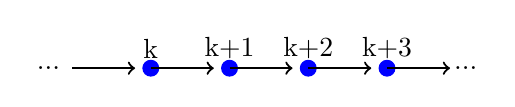
\begin{tikzpicture}
		
		\node[] at (-1.3,0) {...};
		\node[] at (4,0) {...};
		
		\filldraw[fill=blue,draw=blue] (0,0) circle (0.1cm) node[above] {k};
		\filldraw[fill=blue,draw=blue] (1,0) circle (0.1cm) node[above] {k+1};
		\filldraw[fill=blue,draw=blue] (2,0) circle (0.1cm) node[above] {k+2};
		\filldraw[fill=blue,draw=blue] (3,0) circle (0.1cm) node[above] {k+3};
		\draw[->, thick] (0,0) -- (0.8,0);
		\draw[->, thick] (-1,0) -- (-0.2,0);
		\draw[->, thick] (1,0) -- (1.8,0);
		\draw[->, thick] (2,0) -- (2.8,0);
		\draw[->, thick] (3,0) -- (3.8,0);
		
		
	\end{tikzpicture}

    \begin{equation}
    	\dot{x}_k=F(x_k)+\epsilon Bx_{k-1} \qquad x\in\mathbb{R}^n
    	\label{diffeqinteragenti}
   \end{equation}	
\end{center} 
Come vedremo questo tipo di sistemi può rappresentare per esempio il moto delle macchine sulla strada, dove ogni particella è una macchina e regola la sua velocità in base al comportamento della macchina che ha subito davanti, ma anche una serie di neuroni soggetti ad un impulso esterno che è direttamente fornito dal neurone precedente.\\

Chiediamoci ora se è possibile trasmettere perturbazioni nel sistema da una particella ad un'altra e se si quale vaore di $\epsilon$ lo consente. Osserviamo quindi che la nostra richiesta è del tutto analoga alla richiesta di trasmettere un'onda nel sistema, per cui se definiamo un parametro $\Delta$ che quantifica la "distanza" tra due particelle allora la soluzione deve essere nella forma:
\begin{equation}
	x_k(t)=u(k\Delta - t)
	\label{conditioonda}
\end{equation}
Chiaramente se chiamiamo $u^*$ un preciso valore della soluzione questo è univocamente determinato dal suo argomento che però è dipendente sia dall'indice della particella considerata sia dal tempo, per cui per mantenere l'argomento della funzione costante al variare del tempo dovrò anche variare k permettendo così a $u^*$ di propagarsi nel sistema come un fronte d'onda. \\Solitamente la ricerca di questa soluzione particolare è giustificata dall' osservazione di dinamiche ondulatorie nel sistema.\\

Procediamo quindi sostituendo la (\ref{conditioonda}) nella (\ref{diffeqinteragenti}) in maniera tale da ottenere una \textbf{equazione differenziale con ritardo}, questo tipo di equazioni non è solitamente di facile risoluzione poichè presentano un numero di gradi di libertà non numerabile dovuto alla dipendenza della derivata dalle condizioni ad un tempo precedente $t'-\Delta$. Nella fattispecie osserviamo che $x_{k-1}=u((k-1)\Delta+t)$ ed introducendo la variabile $t'=k\Delta-t$ abbiamo:
\begin{equation*}
		\dot{x}_k=\dot{u}=F(u)+\epsilon Bu(k\Delta+t-\Delta)
\end{equation*}
\paragraph{Equazione differenziale con ritardo}
\begin{equation}
	\dot{u}=F(u)+\epsilon Bu(t'-\Delta) \label{eqdiffritardo}
\end{equation}
Se a questo punto la (\ref{eqdiffritardo}) risulta lineare o è linearizzabile possiamo cercare una sua soluzione nella forma esponenziale dipendente degli autovalori di una matrice. 
\begin{equation*}
	u(t)=\sum v_\lambda e^{\lambda t}\qquad \Rightarrow \qquad  \lambda v_\lambda = (A+\epsilon Be^{-\Delta\lambda})v_\lambda
\end{equation*}
Inserendo la ipotizzata soluzione nella (\ref{eqdiffritardo}) scopriamo che gli autovalori sono della matrice $A+\epsilon Be^{-\Delta\lambda}$, per è chiaro dall'algebra lineare che possiamo trovarli e quindi risolvere l'equazione differenziale, tramite la risluzione del polinomio caratteristico dato dal determinate della matrice che abbiamo ottenuto:
\begin{equation}
	\det(\lambda I-A-\epsilon Be^{-\Delta \lambda})=0
\end{equation}

Consideriamo ora le particelle non più collegate in maniera sequenziale ma a formare una grafo dove ogni particella è un nodo collegata ad altri con dei link che consentano di interagire in entrambe le direzioni. Possiamo definire la \textbf{matrice di adiacenza} $A_{ij}$ che assume il valore $1$ se tra la particella i-esima e j-esima vi è un link e "0" altrimenti. Così facendo la (\ref{diffeqinteragenti})
diventa:
\begin{equation}
		\dot{x}_k=F(x_k)+\epsilon \sum A_{kh} x_h
\end{equation}
Questa tipologia di equazioni differenziali può essere ulteriormente modificato affinchè le interazioni, che possono essere viste come scambi di una certa quantità tra una particella ed un'altra, abbiano un senso più fisico, ossia che la quantità scambiata, in analogia con l'impulso, sia conservata. Per far ciò introduciamo il vettore $D_i=\sum A_{ij}$ che assume il valore esatto di link che possiede un determinato nodo, questa matrice ci consente di aggiungere un termine di "conservazione":
\begin{equation}
	\dot{x}_k=F(x_k)+\epsilon \sum( A_{kh} x_h-\delta_{hk}D_kx_k)
\end{equation}
\paragraph{Matrice laplaciana}
Il termine di interazione così costruito trasferisce una quantità dinamica alle particelle collegate attraverso la matrice di adiacenza e ne sottrae una pari quantità alla particella k-esima, attraverso il vettore $D_k$, così che ne complesso si abbia conservazione. Il termine complessivo di interazione prende quindi il nome di \textbf{matrice laplaciana}:
\begin{equation}
	L_{kh}=-( A_{kh}-\delta_{hk}D_k)
\end{equation}
Queste matrici svolgono il ruolo discreto dell'operatore laplciano e risultano dunque estremamente utili per lo studio dei sistemi interagenti, delle loro numerose proprietà ne citiamo le più importanti:
\begin{itemize}
	\item L è simmetrica
	\item Se L ha più di un autovalore nullo il grafo è separabile in due sottosistemi distinti
	\item Se il grafo non è separabile ho tutti autovalori positivi tranne uno nullo che ha sempre l'autovettore associato $v_\lambda=(1,1,1,...)$.
\end{itemize}
\subsection{Sincronizzazione di sistemi intergaenti}
\begin{center}
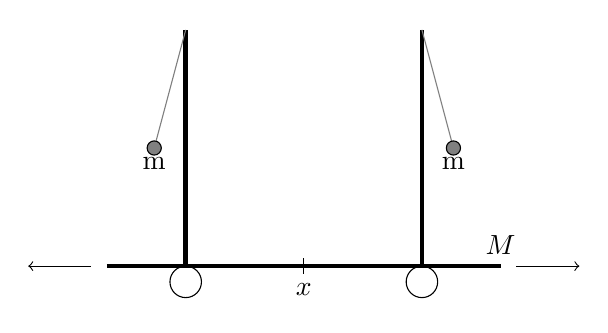
\begin{tikzpicture}
	\draw[ultra thick] (0,0) -- (5,0) node[above] {$M$};
	\draw (1,-0.2) circle (0.2cm);
	\draw (4,-0.2) circle (0.2cm);
	\draw[<-] (-1,0) -- (-0.2,0);
	\draw[->] (5.2,0) -- (6,0);
	\draw (2.5,0.1) -- (2.5,-0.1)  node[below] {$x$};
	\draw[ultra thick] (1,0) -- (1,3);
	\draw[ultra thick] (4,0) -- (4,3);
	\draw[draw=gray] (1,3) -- (0.6,1.5);
	\filldraw[fill=gray] (0.6,1.5) circle (0.09cm) node[below] {m};
		\draw[draw=gray] (4,3) -- (4.4,1.5);
	\filldraw[fill=gray] (4.4,1.5) circle (0.09cm) node[below] {m};
	
\end{tikzpicture}
\end{center}
Per analizzare il problema della sincronizzazione proviamo a studiare il sistema meccanico rappresentato sopra, costituito da due pendoli di massa $m$ legati ad un filo di lunghezza $l$ e vincolati su una base basculante di massa $M$, si osserva sperimentalmente che questo tipo di sistema si sincronizza in maniera tale che, seppur partendo da fasi differenti, le oscillazioni dei due pendoli tendano ad un moto sincrono controfase. Per cominciare scriviamo la lagrangiana del sistema:
\begin{equation}
	\mathcal{L}=\frac{M}{2}\dot{x}^2+\frac{m}{2}(2\dot{x}^2+\dot{\theta_1}^2l^2+\dot{\theta_2}^2l^2+2\dot{x}l(\dot{\theta_1}\cos\theta_1+\dot{\theta_2}\cos\theta_2))+mgl(\cos\theta_1+\cos\theta_2)
\end{equation}
conoscendo quest'ultima possiamo descrivere l'evoluzione dinamica dei pendoli, osserviamo però che questo sistema, nelle ipotesi ideali che stiamo assumendo implicitamente, non può sincronizzarsi, infatti una proprietà dei sistemi dinamici \textit{Hamiltoniani} è la reversibilità che verrebbe a mancare se avvenisse la sincronizzazione: infatti giunti alla condizione di moto sincrono non si sarebbe più in grado si risalire alle condizioni iniziali.\\
Siamo infatti costretti a considerare gli attriti così da non studiare più un sistema reversibile, per cui procediamo in primis considerando il regime delle piccole oscillazioni:
\begin{equation}
	\mathcal{L}_{po}=\frac{M}{2}\dot{x}^2+\frac{m}{2}(2\dot{x}^2+\dot{\theta_1}^2l^2+\dot{\theta_2}^2l^2+2\dot{x}l(\dot{\theta_1}+\dot{\theta_2}))-\frac{mgl}{2}(\theta_1^2+\theta_2^2)
\end{equation}
Osserviamo che $x$ è una coordinata ciclica per cui è il suo momento associato è un integrale primo del moto da cui abbiamo $\dot{x}=-l\frac{m}{2m+M}(\dot{\theta_1}+\dot{\theta_2})$ che ci consente di ridurre i gradi di livertà del problema e di ricondurci ad una lagrangiana data da sole forme quadratiche, infatti se chiamiamo $a=\frac{m}{2m+M}$ tramite qualche passaggio algebrico abbiamo:
\begin{equation*}
   \begin{gathered}
   	\mathcal{L}_{po}=l^2\frac{m}{2}(1-a)(\dot{\theta_1}^2+\dot{\theta_2}^2)+2ml^2a(a-1)\dot{\theta_1}\dot{\theta_2}-\frac{mgl}{2}(\theta_1^2+\theta_2^2)\\
   	\mathcal{L}_{po}=l^2\frac{m}{2}(1-a)
   	\begin{pmatrix}
   		\dot{\theta_1} \\
   		\dot{\theta_2}
   	\end{pmatrix}
   \begin{pmatrix}
   	1 & -2a \\
   	-2a & 1
   \end{pmatrix} 
   \begin{pmatrix}
   	\dot{\theta_1} \\
   	\dot{\theta_2}
   \end{pmatrix}
   -\frac{mgl}{2}
   \begin{pmatrix}
   	\theta_1 \\
   	\theta_2
   \end{pmatrix}
   I
   \begin{pmatrix}
   	\theta_1 \\
   	\theta_2
   \end{pmatrix}
   \end{gathered}	
\end{equation*}
utilizzando le equazioni di eulero-lagrange otteniamo il sistema di equazioni differenziali:
\begin{equation*}
	\begin{gathered}
		l^2m(1-a)
		\begin{pmatrix}
			1 & -2a \\
			-2a & 1
		\end{pmatrix}
	\begin{pmatrix}
		\ddot{\theta_1} \\
		\ddot{\theta_2}
	\end{pmatrix}
    =-mgl
    \begin{pmatrix}
    	\theta_1 \\
    	\theta_2
    \end{pmatrix}
	\end{gathered}	
\end{equation*}
introduciamo un termine d'attrito:
\begin{equation*}
	\begin{gathered}
		l^2m(1-a)
		\begin{pmatrix}
			1 & -2a \\
			-2a & 1
		\end{pmatrix}
		\begin{pmatrix}
			\ddot{\theta_1} \\
			\ddot{\theta_2}
		\end{pmatrix}
		=-\gamma
			\begin{pmatrix}
			\ddot{\theta_1} \\
			\ddot{\theta_2}
		\end{pmatrix}
		-mgl
		\begin{pmatrix}
			\theta_1 \\
			\theta_2
		\end{pmatrix}
	\end{gathered}	
\end{equation*}
Se diagonaliziamo la matrice metrica dell'energia cinetica troviamo due autovettori con due auto valori, le combinazioni lineari delle soluzioni del sistema secondo questi due autovettori ci danno la generica soluzione per cui:
\begin{itemize}
	\item $\lambda=1-2a$ con $v_{\lambda}=(1,1)$, che da un sistema oscillante in fase che è descritto dall'equazione:
	\begin{equation*}
			\begin{pmatrix}
				\ddot{\theta_1} \\
				\ddot{\theta_2}
			\end{pmatrix}
			=-\frac{\gamma}{l^2m(1-a)(1-2a)}
			\begin{pmatrix}
				\ddot{\theta_1} \\
				\ddot{\theta_2}
			\end{pmatrix}
			-\frac{g}{l(1-a)(1-2a)}
			\begin{pmatrix}
				\theta_1 \\
				\theta_2
			\end{pmatrix}
	\end{equation*}
In questo caso poichè $a=\frac{m}{2m+M}$ per $M\rightarrow0$ abbiamo che $a\rightarrow\frac{1}{2}$ il termine dissipativo diventa infinitamente grande, per cui questa soluzione se presente si dissipa molto rapidamente se la massa della base è molto piccola.
\item $\lambda=1+2a$ con $v_{\lambda}=(1,-1)$, che da un sistema oscillante in controfase che è descritto dall'equazione:
\begin{equation*}
	\begin{pmatrix}
		\ddot{\theta_1} \\
		\ddot{\theta_2}
	\end{pmatrix}
	=-\frac{\gamma}{l^2m(1-a)(1+2a)}
	\begin{pmatrix}
		\ddot{\theta_1} \\
		\ddot{\theta_2}
	\end{pmatrix}
	-\frac{g}{l(1-a)(1+2a)}
	\begin{pmatrix}
		\theta_1 \\
		\theta_2
	\end{pmatrix}
\end{equation*}
Con lo stesso ragionamento del punto precedente osserviamo che il termine dissipativo non cresce rapidamente come nel caso in fase il che consente a questo modo di manifestarsi nella dinamica del sistema che risulterà quindi sincronizzato.
\end{itemize} 

\bibliographystyle{plain}
\bibliography{ref}

\end{document}
